% Chapter 5

\chapter{Diseño} % Main chapter title

\label{Chapter5} % Change X to a consecutive number; for referencing this chapter elsewhere, use \ref{ChapterX}

%Intro del capitulo
En este capítulo se muestra el diseño del simulador programado. El objetivo  de esta sección fue crear un modelo de sistema, para el cual se especificó un escenario y el modelado de cuatro principales componentes que acabaron siendo implementados en el simulador: el despliegue de UEs, el modelo de canal, el esquema de acceso al múltiple al medio y los modelos de tráfico.\newline

%----------------------------------------------------------------------------------------
%	SECTION 
%----------------------------------------------------------------------------------------

\section{MODELO DE SISTEMA}

En principio, se comenzó con la etapa de análisis (\textit{Capítulo \ref{Chapter4}}), donde se analizaron los requisitos de la red, las características que debía tener el escenario que se propuso y los distintos modelos que formaron parte de la simulación.\newline

En términos generales, se consideró una red celular uni-celda para transmisiones de subida (\textit{uplink}), el escenario se trata de uno urbano macro celular (UMa) en donde frecuentemente los UEs se situan estáticos y en el exterior. De acuerdo a los modelos analizados y ya elegidos en la \textit{Sección~\ref{AnalisisMODELOS}}, el modelo de sistema del simulador  implementó los siguientes sub-sistemas \textit{[Figura~\ref{fig:DiagramaGral}]}:

\begin{enumerate}
    \item  Uso de una geometría estocástica, es decir, despliegue de UEs siguiendo un PPP.
    \item  Pérdidas de canal usando un modelo CI para ambientes exteriores.
    \item  Incorporación de un esquema de acceso al medio no ortogonal (NOMA) usando una técnica de agrupamiento \textit{(clustering)} de usuarios.
    \item  Diferentes modelos de tráfico que simulen distintos servicios para NB-IoT.
\end{enumerate}

\begin{figure}[th]
    \centering
    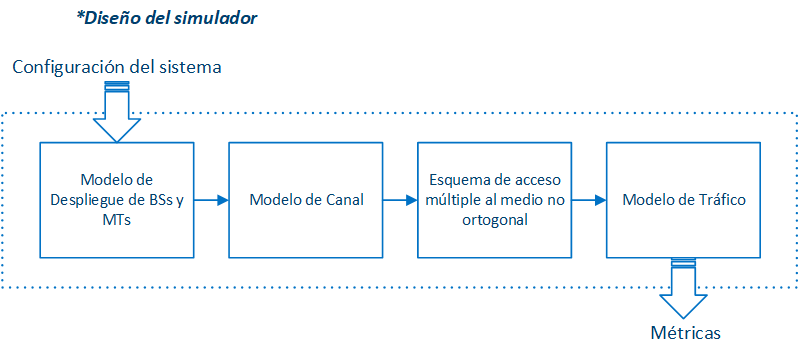
\includegraphics[scale=.9]{Figures/Diagrama general de bloques del simulador}
    \decoRule
    \caption[Diagrama general de bloques del simulador, constando principalmente de 4 módulos.]{Diagrama general de bloques del simulador, constando principalmente de 4 módulos.}
    \label{fig:DiagramaGral}
\end{figure}

El simulador se enfocó en el caso de uso de mMTC (o mIoT) el cual se caracteriza por brindar servicio a un gran número de dispositivos, esto es, teniendo una alta densidad de volumen de tráfico en escenarios con aglomeración de dispositivos. Por lo tanto, como se revisó en el capítulo anterior un excelente candidato para cumplir con los requerimientos del caso de uso mIoT y que forma ahora parte del estándar 5G, fue la tecnología NB-IoT. De este estándar, se tomaron sus especificaciones técnicas (\textit{Sección~\ref{NBIoT} }), tales como los parámetros fundamentales para la comunicación entre la BS y los UEs en la simulación.\newline

A continuación se definen las características generales de cada sub-sistema:

\subsection{Uso de una geometría estocástica, es decir, despliegue de UEs siguiendo un PPP}

De igual manera que se realizó en \parencite{Kouzayha2018} y \parencite{Zhang2017} con el fin de obtener un análisis fundamental y más realista, se propuso la generación de una geometría estocástica en 2D para la distribución de los UEs. Se tomó como modelo de despliegue de UE un \textit{ Homogeneous Poisson Point Process }(proceso puntual de Poisson homogeneo, HPPP) con distintas densidades para los diferentes tipos de dispositivos que se implementaron.\newline

\subsection{Pérdidas de canal usando un modelo CI para ambientes exteriores}

En la \textit{Sección \ref{AppsEscenario} } se establecieron las aplicaciones de los diferentes dominios de IoT que se utilizaron en el simulador. Todas estas aplicaciones se encuentran presentes, no exclusivamente pero sí particularmente, en escenarios urbanos y en exteriores, por lo tanto se implementó el Modelo CI (ecuación \ref{eqn:CI} ) el cual de acuerdo a lo estudiado en \parencite{Sun2016} es el modelo que mejor estima la señal en este tipo de ambientes. Además, se agregarón perdidas por el desvanecimiento rápido, usando el modelo de desvanecimiento de Rayleigh (siguiendo una distribución Rayleiggh con desviación estándar unitaria y que se distribuyó de forma independiente e idéntica [i.i.d.]), este es ideal para entornos urbanos en situaciones donde hay un gran número de multi-trayectorias de la señal y reflexiones causadas por los edificios y objetos que obstruyen la línea de vista. \newline

Con base en \parencite{Sun2016}, para el Modelo CI en ambientes urban macro se tienen los parámetros mostrados en la Tabla~\ref{tab:ModeloCI} que dependiendo el tipo de ambiente (ya sea con línea de vista [LoS] o sin línea de vista [NLoS]) los parámetros rango de distancia y el exponente de pérdida (PLE) varían. El modelo de sistema propuesto se trata de un ambiente en exteriores, se considera que sí habrá línea de vista entre los UE y la BS, por lo tanto, se utilizó LoS con distancias entre [60 - 900 m] y un PLE igual a 2.\newline
\begin{table}
    \caption{Parámetros Modelo CI [Fuente: \parencite{Sun2016}]}
    \label{tab:ModeloCI}    
    \centering
    \begin{tabular}{*{7}{m{2cm}}}\\ 
    \textbf{Escenario} & \textbf{Ambiente} & \textbf{Rango de Frecuencias} & \textbf{\# Puntos de Datos\newline analizados} & \textbf{Rango de distancias\newline entre BS y UE} & \textbf{Modelo Canal} & \textbf{PLE} \\ \midrule
    \multirow{2}{*}{\textbf{\begin{tabular}[c]{@{}c@{}}UMa\end{tabular}}} & \textit{LoS} & \textit{2 - 38 GHz} & \textit{1032} & \textit{60 - 930 m} & \textit{CI} & \textit{2.0} \\
     & \textit{NLoS} & \textit{2 - 38 GHz} & \textit{1869} & \textit{61 - 1238 m} & \textit{CI} & \textit{2.9} \\ \cmidrule(l){2-7} 
    \end{tabular}
\end{table}

Algunos parámetros siguieron las características de las mediciones que se hicieron para validar el modelo CI, en \parencite{Sun2016}. Las mediciones se realizaron en Vestby, Aalborg, Dinamarca, en las bandas de frecuencia de 2, 10, 18 y 28 GHz en marzo. Vestby representa una típica ciudad europea de tamaño mediano con construcciones y anchos de calle regulares, que son de aproximadamente 17 m (cinco pisos) y 20 m, respectivamente. Para el escenario UMa, la antena BS está por encima de la altura de la azotea, típicamente 25 m más o menos por encima del suelo \parencite{Sun2016}.\newline

Por último, para la definición del rango de frecuencia de las transmisiones, como se pudó leer en la Sección~\ref{NBIoT}, en la actualidad el despliegue de redes NB-IoT se ha realizado en bandas EUTRA (Acceso de radio en LTE) y bandas GSM (SA), por lo que este sistema se implementó en la banda de microondas, se ocupó la banda mas baja en la cual el modelo CI es válido, es decir, la banda de 2GHz.

\subsection{Incorporación de un esquema de acceso al medio no ortogonal (NOMA) usando una técnica de agrupamiento de usuarios}
Se predefinió que exista un bloque de recursos (PRB) para la BS dedicado para el estándar NB-IoT en la banda de 2GHz, dando servicio a comunicaciones tipo maquina (MTC). El recurso de radio tiene un ancho de banda de 180kHz y este recurso se dividió en 48 sub-portadoras de 3.75kHz con operación \textit{singletone y multitone}.\newline

Por lo tanto, para la compartición de recursos, en vías de dar servicio a un gran número de dispositivos, propuso implementar un esquema de acceso múltiple al medio no ortogonal (NOMA) descrito en la \textit{Sección~\ref{NOMA_C4}} y la implementación de una técnica de agrupamiento de usuarios (\textit{clustering}) y se aprovechará la no ortogonalidad, para agrupar diferentes clases de nodos IoT en una misma sub-banda.\newline

En este caso como consideraremos dos tipos de sensores los mMTC y los URLLC, (con mayores requisitos de transmisión de datos los segundos). La relación de la distribución de dispositivos mMTC con los URLLC fue de 3 a 1.\newline

El cálculo de las tasas de los dispositivos URLLC y mMTC, se describen con las Ecuaciones~\ref{eqn:Ru} y ~\ref{eqn:Rm} respectivamente.\newline

Con la incorporacion del Modelo de Canal CI, el cálculo de las ganancias $h$ se dió de la siguiente manera:

\begin{equation}
    h =  10^{(\frac{-L_{p [dB]}^{CI}}{10})} \cdot \gamma\ [W]
    \label{eqn:h_canal}
\end{equation}
Donde:
\[\gamma \to ganancia\ desvanecimiento\ Rayleigh\]
\[\ L_{p [dB]}^{CI} \to \textit{Path\ Loss}\ Modelo\ CI \]

\subsection{Diferentes modelos de tráfico que simulen distintos servicios para NB-IoT}

En la implementación de modelos de tráfico se tuvo en cuenta el modelo CMMPP y un modelo determinístico. El modelo CMMPP pudo tener una instancia distinta para cada una de las aplicaciones que se propusieron en \textit{Tabla~\ref{tab:appssim} } a excepción de aquellas aplicaciones con transmisiones periódicas, para las cuales se utilizó un modelo determinístico\textit{.}\newline

Cada tipo de dispositivo tiene una instancia de \textit{procesos maestros}. Estos procesos, están modificando las probabilidades de cambio de estado de cada nodo según su proximidad a otros nodos que estén cambiando de estado. Por ejemplo, digamos que un nodo, que llamaremos N1, que detecta terremotos se encuentra en estado de reposo y su probabilidad de transición al estado de transmisión por alarma es del 1\%, ahora de pronto otro nodo (de la misma aplicación) en su proximidad cambia de estado a transmisión por evento, y unos instantes después la probabilidad de transición en nuestro nodo que antes era del 1\% aumenta hasta 90\%, lo que desencadena que este nodo también comience a transmitir al cambiar de estado unos momentos después. El ejemplo anterior, en la vida real se traduciría como un terremoto ocurriendo en un lugar y una gran cantidad de nodos que se encargan de detectarlo comenzando de pronto a transmitir con una indudable coordinación espacial y temporal.\newline

\begin{figure}[th]
\centering
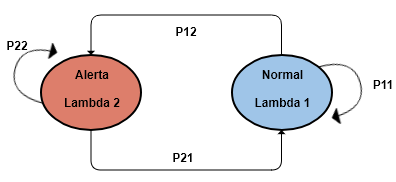
\includegraphics[scale=1]{Figures/Cadena de Markov propuesta}
\decoRule
\caption[Cadena de Markov propuesta]{Cadena de Markov propuesta}
\label{fig:CMMPPpropuesta}
\end{figure}

Habiendo explicado esto, la implementación del modelo CMMPP en las aplicaciones, control de iluminación, detección de terremotos y genérico contará con un diseño de cadena de Markov como el que se presenta en la \textit{Figura~\ref{fig:}. }En esta figura se puede ver que se modelarán dos distintos estados para cada nodo IoT de estas aplicaciones. El primer estado, llamado normal corresponde al funcionamiento \textbf{normal} o principal de la aplicación, con una tasa de transmisión Lambda 1 (${\lambda }_1$). A la vez el segundo estado, llamado \textbf{Alerta} o Alarma con tasa de transmisión Lambda 2 (${\lambda }_2$), corresponde al estado que acudirán los dispositivos IoT de acuerdo con eventos de interes producidos aleatoriamente en el área de la célula. Es justamente con la ayuda de este estado que el modelo es capaz de simular la coordinación espacial y temporal de los dispositivos.

\begin{equation}
P_n\left[k\right]=\ _n\left[k\right] P_c+\left(1-\ _n\left[k\right]\right)\ P_u 
\label{eqn:Pn}
\end{equation}

\[donde:\ n\ corresponde\ al\ n-\textrm{é}simo\ nodo\] 
\[y\ k\ a\ un\ determinado\ instante\ de\ tiempo\] 

En la ecuación \ref{eqn:Pn} vemos la forma en la que se modulan las matrices de probabilidad de transición entre los estados. Entonces para calcular la matriz $P_n\left[k\right]$, es decir la perteneciente al nodo \textit{n }en el instante \textit{k, }necesitamos de las matrices $P_c$ y $P_u$ que corresponden al comportamiento coordinado y no coordinado respectivamente y del valor $_n\left[k\right]$. Las matrices $P_c$ y $P_u$ marcan el comportamiento que tendría el nodo en los casos extremos de coordinación o en la ausencia de esta, esto debido a que $_n\left[k\right]$ varía entre [0 ,1], entonces si existe una perfecta coordinación entre nodos y este valor es 1, en algún momento, el segundo sumando de la ecuación \ref{eqn:Pn} sería 0 y $P_n\left[k\right]=\ P_c$. La propuesta para $P_c$ y $P_u$, tal y como se ha utilizado en \parencite{Gupta2018} y \parencite{Smiljkovic2014} fue:

\begin{equation}
P_{u} =  
\begin{bmatrix}
1 & 1 \\
0 & 0 
\end{bmatrix}
\end{equation}

\begin{equation}
P_{c} = 
\begin{bmatrix}
0 & 1 \\
1 & 0 
\end{bmatrix}
\end{equation}

Ahora se estudia el término $_n\left[k\right]$ que es el que se encarga de simular la correlación existente entre los nodos, el cual se compone de $_n\left[k\right]=\ {\delta }_n[k]$, siendo ${\delta }_n$ el término encargado de la coordinación espacial y $[k]$ el de la coordinación temporal. Para ${\delta }_n$ se utilizaron dos funcioness: una exponencial decreciente \textit{Decaying exponential} y una ventana de coseno alzado \textit{Rised-cosine window} según convino para cada aplicación, tal y como se propone en \parencite{Gupta2018}.  La ventana de coseno alzado permitió simular un término abrupto en la transmsión de las alarmas. Finalmente para $[k]$ se calculó su valor utilizando una función delta, que sólo toma el valor 1 cuando la alarma se ha propagado hasta el sitio del nodo. \newline

Mientras un nodo se encuentre en el estado normal, este genera paquetes a la tasa $\lambda_{normal}$. Un cambio de estado se da por una alarma que se propagó hasta el sitio del nodo. En la \textit{Figura~\ref{fig:CMMPP_Algoritmo}} se presenta el diagrama de flujo con el algoritmo que se utilizó como base para generar el tráfico que sigue este modelo, hizo falta la incorporación de tráfico periódico para las aplicaciones que así lo requirieron.\newline

\begin{figure}[th]
\centering
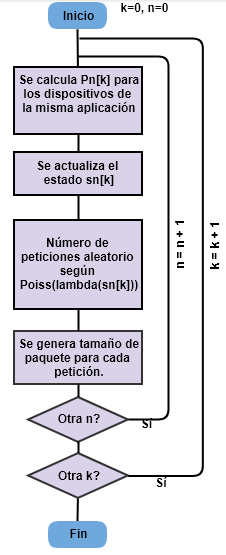
\includegraphics[scale=.7]{Figures/Generación de tráfico con modelo CMMPP}
\decoRule
\caption[Generación de tráfico con modelo CMMPP]{Generación de tráfico con modelo CMMPP}
\label{fig:CMMPP_Algoritmo}
\end{figure}

El segundo modelo se trata de uno determinístico, y fué el que se implementó en las aplicaciones cuya tasa de tráfico es periódica. De manera que lo único que se debe conocer es la tasa de tráfico de los nodos con la cual se calendarizan los nacimientos de paquetes. Las aplicaciones contempladas para este modelo son: el monitoreo del consumo de agua y electricidad en la ciudad, el monitoreo de la contaminación del aire y el control dinámico de los semáforos.\newline

\begin{table}
\caption{Caracterización de las aplicaciones seleccionadas}
\label{tab:AppsSimulacion}
\centering
\begin{tabular}{|p{1.4in}|p{0.7in}|p{0.7in}|p{0.7in}|p{0.4in}|p{1.8in}|} \\ 
\textbf{\textit{Número de Servicio y Nombre}} & \textbf{Tamaño de red} & \textbf{Tasa de tráfico} & \textbf{Demanda de QoS} & \textbf{Clase} & \textbf{Tamaño de paquete} \\ \hline \hline
\textit{1 - Control de iluminación\newline (Ciudad Inteligente) } & \footnotesize{ Grande, miles de dispositivos } & \footnotesize{ Aleatorio, poco frecuente } & \footnotesize{ Media, tolerante al retardo 15seg } & \footnotesize{ mMTC } & \footnotesize{ Activación aleatoria\newline \textbf{UL}: 20 bytes \textit{payload}\newline \textbf{DL}: ACK de 0 bytes } \\ \hline 
\textit{2 - Monitoreo del consumo de agua y electricidad en la ciudad\newline (Ciudad Inteligente) } & \footnotesize{ Media a grande, cientos a miles de dispositivos } & \footnotesize{ Periódico, 1 msj cada 10 min por dispositivo } & \footnotesize{ Baja, tolerante al retardo 1min } & \footnotesize{ mMTC } & \footnotesize{ Activación periódica\newline \textbf{UL}: distribución de Pareto con parámetro alfa = 2.5 y tamaño mínimo de carga útil de la aplicación = 20 bytes con un corte a 200 bytes\newline \textbf{DL}: ACK de 0 bytes 50\% de las veces. } \\ \hline 
\textit{3 - Detección de terremotos\newline (Ambiente Inteligente) } & \footnotesize{ Media a grande, cientos a miles de dispositivos } & \footnotesize{ Aleatorio, poco frecuente } & \footnotesize{ Alta, tolerante al retardo 3seg } & \footnotesize{ mMTC } & \footnotesize{ Activación aleatoria\newline \textbf{UL}: 20 bytes \textit{payload}\newline \textbf{DL}: ACK de 0 bytes } \\ \hline 
\textit{4 - Monitoreo de contaminación del aire\newline (Ambiente Inteligente) } & \footnotesize{ Media a grande, cientos a miles de dispositivos } & \footnotesize{ Periódico, 1 msj cada 15 min por dispositivo } & \footnotesize{ Media, tolerante al retardo 15seg } & \footnotesize{ mMTC } & \footnotesize{ Activación periódica\newline \textbf{UL}: distribución de Pareto con parámetro alfa = 2.5 y tamaño mínimo de carga útil de la aplicación = 20 bytes con un corte a 200 bytes\newline \textbf{DL}: ACK de 0 bytes 50\% de las veces. } \\ \hline 
\textit{5 - Control dinámico de semáforos\newline (Transporte y Movilidad Inteligentes) } & \footnotesize{ Grande, miles de dispositivos } & \footnotesize{ Periódico, 1 msj cada min por dispositivo } & \footnotesize{ Alta, tolerante al retardo 5seg } & \footnotesize{ mMTC } & \footnotesize{ Activación periódica\newline \textbf{UL}: distribución de Pareto con parámetro alfa = 2.5 y tamaño mínimo de carga útil de la aplicación = 20 bytes con un corte a 200 bytes\newline \textbf{DL}: ACK de 0 bytes 50\% de las veces. } \\ \hline 
\textit{6 - Otros Dispositivos mMTC}  & \footnotesize{ Grande, miles de dispositivos } & \footnotesize{ Aleatorio, poco frecuente } & \footnotesize{ Alta, tolerante al retardo 5seg } & \footnotesize{ mMTC } & \footnotesize{ Activación aleatoria\newline \textbf{UL}: 20 bytes \textit{payload}\newline \textbf{DL}: ACK de 0 bytes } \\ \hline 
\textit{7 - Dispositivos URLLC}  & \footnotesize{ Grande, miles de dispositivos } & \footnotesize{ Aleatorio, poco frecuente } & \footnotesize{ Alta, tolerante al retardo 3seg } & \footnotesize{ URLLC } & \footnotesize{ Activación aleatoria\newline \textbf{UL}: 20 bytes \textit{payload}\newline \textbf{DL}: ACK de 0 bytes } \\
\end{tabular}
\end{table}

Ahora, en la \textit{Tabla~\ref{tab:AppsSimulacion}} se presentan las aplicaciones mencionadas en la \textit{sección \ref{AppsEscenario}} junto a su caracterización. Adicionalmente se anexó la distinción de las aplicaciones en dos clases distintas, mMTC y URLLC que permitió realizar el algoritmo de agrupaciones NOMA. Se buscó que por cada nodo URLLC hubieran por lo menos 3 nodos mMTC. por lo tanto se utilizaron distintas intensidades de dispositivos que conservaran la relación. \newline


En la \textit{Figura~\ref{fig:EscenarioMTC}} se muestra una aproximación del escenario implementado, usando un agrupamiento con cuatro nodos.

\begin{figure}[th]
\centering
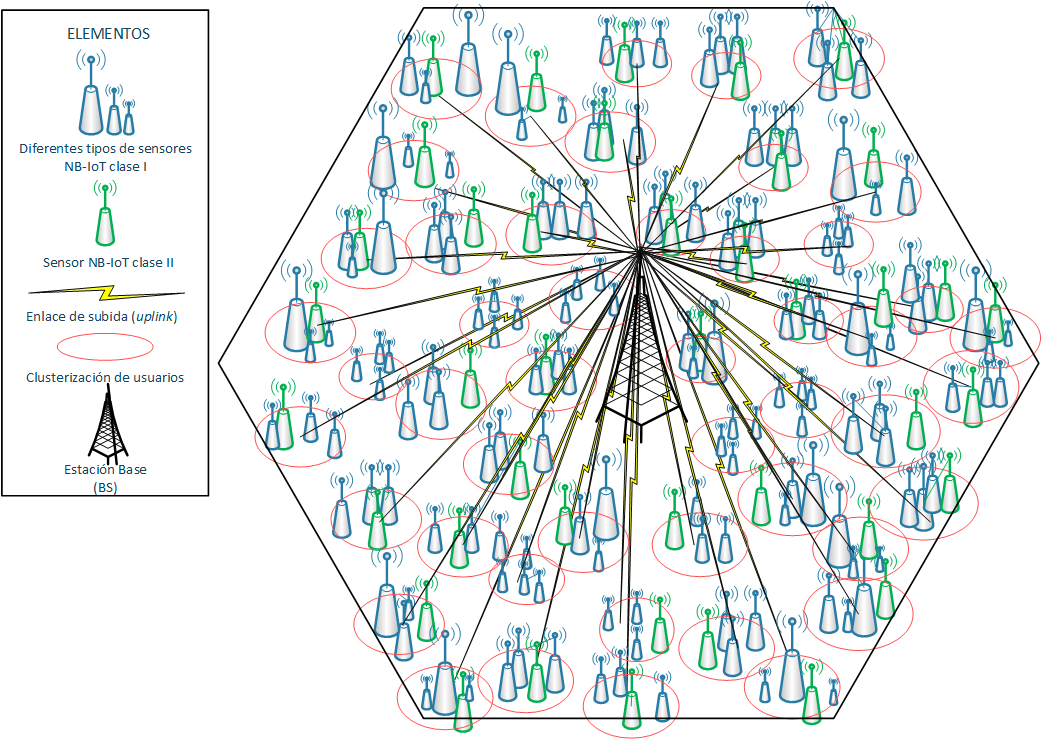
\includegraphics[scale=.65]{Figures/Escenario mIoT unicelda}
\decoRule
\caption[Ejemplo ilustrativo de un escenario mIoT unicelular aproximado, usando agrupaciones de 4 dispositivos]{Ejemplo ilustrativo de un escenario mIoT unicelular aproximado, usando agrupaciones de 4 dispositivos}
\label{fig:EscenarioMTC}
\end{figure}
%%%%%%%%%%%%%%%%%%%%%%%%%%%%%%%%%%%%%%%%%%%%%%%%%%%%%%%%%%%%%%%%%%%%%
\section{Parámetros generales del simulador}\label{parametrossimulador}

Para planear un modelo de sistema válido y coherente se incorporaron algunos parámetros generales de diseño revisados en los artículos \parencite{Shahini2019}, \parencite{Mostafa2019} y \parencite{Gupta2018}. La \textit{Tabla~\ref{tab:ParametrosGral}} describe el conjunto de parámetros de la simulación.

\begin{table}
    \caption{Parámetros de la simulación a nivel de sistema}
    \label{tab:ParametrosGral}
    \centering
    \begin{tabular}{|m{6cm}|p{10cm}|} \\ 
    \textbf{Parámetro} & \textbf{Valor} \\ \hline  \hline 
    \textit{Escenario}  & \footnotesize{ UMa } \\ \hline 
    \textit{Ambiente}  & \footnotesize{ LoS } \\ \hline 
    \textit{Diseño celular}  & \footnotesize{ uni-celular } \\ \hline 
    \textit{Transmisión}  & \footnotesize{ UL } \\ \hline 
    \textit{Radio de celula}  & \footnotesize{ 200 m } \\ \hline 
    \textit{Movilidad de UEs}  & \footnotesize{ Nula - 0km/h } \\ \hline 
    \textit{Distribución de UEs } & \footnotesize{ Procesos puntuales de Poisson Homogeneos (HPPP) } \\ \hline 
    \textit{Modelo de canal de propagación `Path Loss' } & \footnotesize{ Modelo CI\newline $L^{CI}_p(f,d)_{\left[dB\right]}=32.4+\ 10\ n{\ log}_{10}\left(\frac{d}{d_0}\right)+{\ 20\ log}_{10}\left(d_0\right)+{20\ log}_{10}\left(f\right)+x^{CI}_{\sigma .}$ } \\ \hline 
    \textit{PLE}  & \footnotesize{ 2 } \\ \hline 
    \textit{$d_0$}  & \footnotesize{ 1m } \\ \hline 
    \textit{Modelo de Tráfico} & \footnotesize{ CMMPP y Periódico} \\ \hline 
    \textit{Esquema de acceso múltiple al medio } & \footnotesize{ NOMA usando agrupamientos } \\ \hline 
    \textit{Relación entre dispositivos mMTC y uRLLC } & \footnotesize{ 3 a 1 } \\ \hline 
    \textit{$K_{max}$ } & \footnotesize{ 1, 2, 3 y 4 } \\ \hline 
    \textit{Número de antenas BS } & \footnotesize{ 1 } \\ \hline 
    \textit{Número de antenas UE } & \footnotesize{ 1 } \\ \hline 
    \textit{Potencia máxima de transmisión de nodos uRLLC } & \footnotesize{ 23 dBm } \\ \hline 
    \textit{Potencia máxima de transmisión de nodos mMTC } & \footnotesize{ 23, 20 o 14 dBm } \\ \hline 
    \textit{Densidad de Ruido Térmico} & \footnotesize{ -174 dbm/Hz } \\ \hline 
    \textit{Frecuencia de operación}  & \footnotesize{ En banda y guarda de banda LTE estándar,\newline Banda de 2GHz } \\ \hline 
    \textit{Ancho de banda del sistema para un PRB (BW) } & \footnotesize{ 180 KHz } \\ \hline 
    \textit{Espacio entre sub-portadoras Uplink}  & \footnotesize{ 3.75kHz \textit{singletone y multitone} \parencite{Shahini2019}} \\ \hline 
    \textit{Tasa de datos máxima} & \footnotesize{ UL: 20kbps} \\  
    \end{tabular}
\end{table}

Para la generación de variables aleatorias se usaron las librerías \textit{scipy, numpy ó random} en Python.